% no notes
\documentclass[dvipsnames]{beamer}
% notes and slides
%\documentclass[notes]{beamer}
% notes only
% \documentclass[notes=only]{beamer}
\usepackage{graphicx} % Allows including images
\usepackage{booktabs} % Allows the use of \toprule, \midrule and \bottomrule in tables
\usepackage{multirow}
\usepackage{multimedia}
\usepackage{tikz}
\usepackage{circuitikz}
\usepackage{url}
\usepackage{pgfplots}
\pgfplotsset{compat=newest}
\usepgfplotslibrary{groupplots,dateplot}
\usetikzlibrary{patterns,shapes.arrows}
\usepackage{standalone}
\usepackage{adjustbox}
\usepackage{lmodern}
\usepackage{pgfplots}
\usepackage{amsmath}
\usepackage{amsthm}
\usepackage{multimedia}
\usepackage{standalone}
\usepackage{csquotes}
\usepackage{caption}


\DeclareMathOperator*{\argmax}{argmax}
\DeclareMathOperator*{\argmin}{argmin}


\PassOptionsToPackage{american}{babel} % change this to your language(s), main language last
% Spanish languages need extra options in order to work with this template
% \PassOptionsToPackage{spanish,es-lcroman}{babel}
\usepackage{babel}

\newcommand{\referencefootnote}[1]{\setbeamertemplate{footline}[text line]{%%%
\parbox{0.9\paperwidth}{\vspace*{-23pt}\tiny{\textcolor{gray}{#1}}\hfill\scriptsize\insertframenumber}}}

% Redefine the caption format to remove "Figure"
\captionsetup[figure]{labelformat=empty}

\PassOptionsToPackage{%
  backend=biber,bibencoding=utf8, %instead of bibtex
  %backend=bibtex8,bibencoding=ascii,%
  language=auto,%
  style=numeric-comp,%
  %style=authoryear-comp, % Author 1999, 2010
  %bibstyle=authoryear,dashed=false, % dashed: substitute rep. author with ---
  style=alphabetic,
  sorting=nyt, % name, year, title
  maxbibnames=10, % default: 3, et al.
  %backref=true,%
  %natbib=true % natbib compatibility mode (\citep and \citet still work)
}{biblatex}
\usepackage{biblatex}

\addbibresource{bib.bib}

\usetheme{metropolis}           % Use metropolis theme
\setbeamertemplate{caption}[default]
\title{Support Vector Machines}
\date{February 17, 2025}%{\today}
\institute{Visual Computing Group, University of Bonn}
\author{Elena Trunz}

\titlegraphic{
\includegraphics[width=2.00cm]{UNI_Bonn_Logo_Standard_RZ.pdf}}
\begin{document}
    \maketitle

    \begin{frame}
    \frametitle{Overview} 
    \tableofcontents
    \end{frame}

    \section{Introduction}
    \begin{frame}{Classification}
			\emph{Given:} 
			\begin{itemize}
				\item Training data: example-label pairs: $\{(\textbf{x}_1,y_1), \dots, (\textbf{x}_N,y_N)\}$
				\item Inputs $\textbf{x}_i \in \mathbb{R}^m$
				\item Target labels $y_j \in Y = \{t_1, \dots, t_K\}$, $K =$ number of classes %\pause
			\end{itemize}
			
			\emph{Find:} Classifier (\emph{hypothesis}) $f:\mathbb{R}^m \rightarrow Y$, with small generalization error.
    \end{frame}
		
		\begin{frame}{Classification algorithm}
		Idea:
			\begin{enumerate}
				\item Represent input data in $\mathbb{R}^m$ %\pause
				\item Partition the space, such that only the examples with the same label are in the same partition
			\end{enumerate}
    \end{frame}
		
		{ \referencefootnote{Image was taken from \cite{deisenroth_faisal_ong_2020}}
		\begin{frame}{Binary classification}
			Only two classes: $Y = \{-1, +1\}$
			
			 \begin{figure}
					\center
					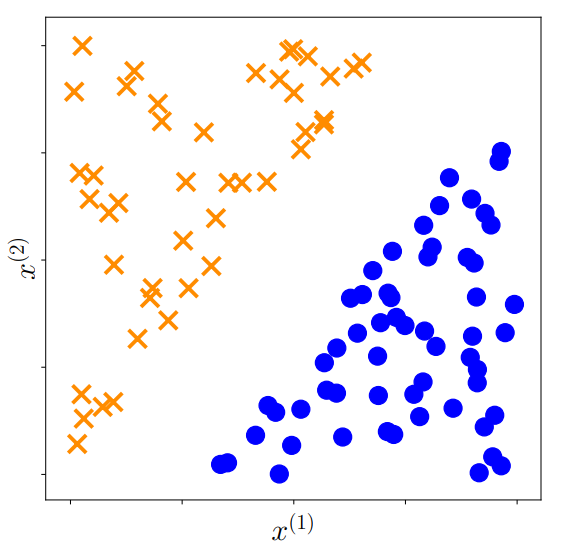
\includegraphics[scale=.35]{figures/binary.png}
           %\caption{2D data from two classes}
        \end{figure}
    \end{frame}
		}
		
		\begin{frame}{What is the best classifier?}
			 \begin{figure}
					\center
					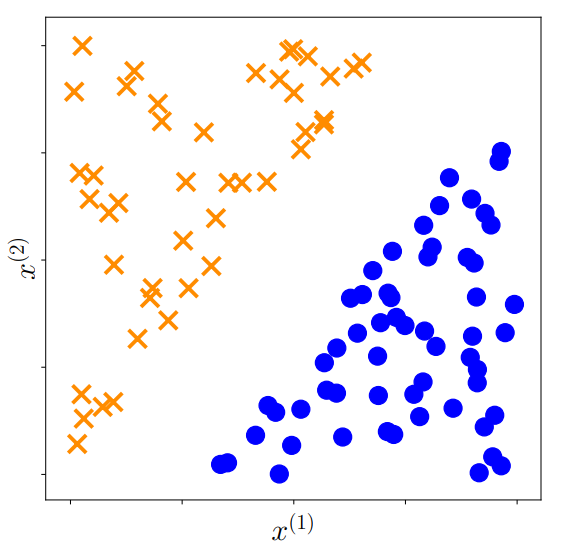
\includegraphics[scale=.35]{figures/binary.png}
        \end{figure}
    \end{frame}
		
		{ \referencefootnote{Image was taken from \cite{deisenroth_faisal_ong_2020}}
			\begin{frame}{What about this data?}
			 \begin{figure}
					\center
					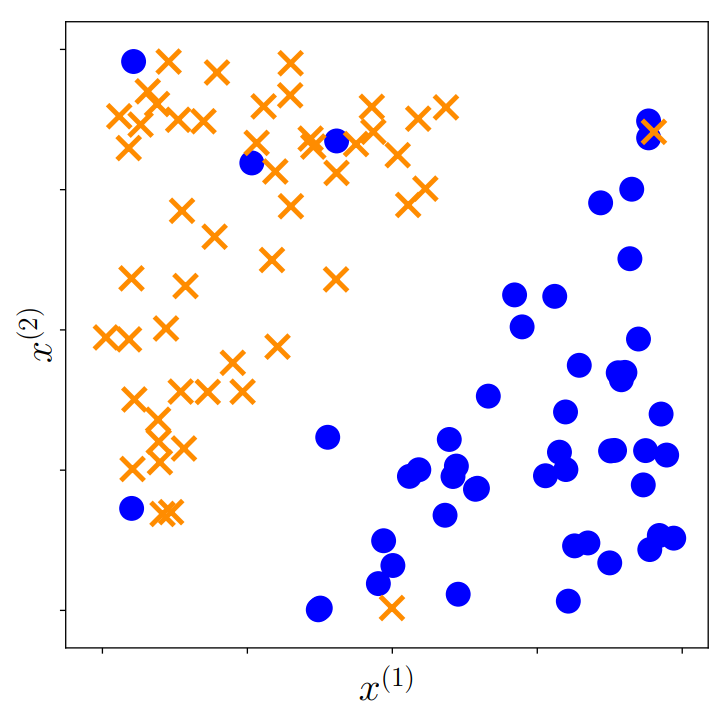
\includegraphics[scale=.28]{figures/binary3.png}
        \end{figure}
    \end{frame}
		}
		
		\section{Linearly Separable Data}
		\begin{frame}{Narrow down the search}
			What is the best classifier here?
				\begin{figure}
					\center
					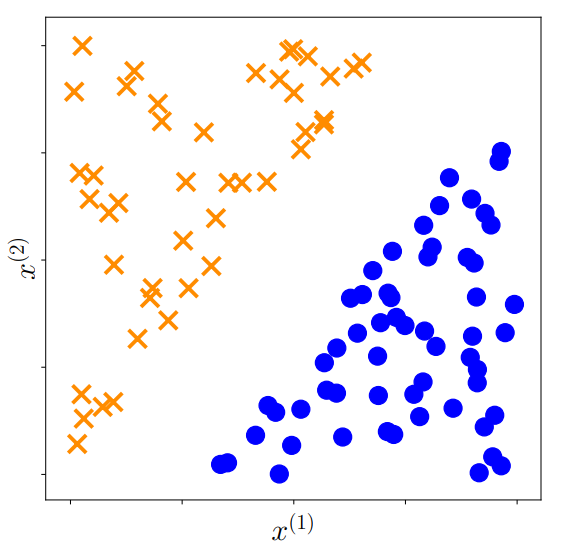
\includegraphics[scale=.3]{figures/binary.png}
        \end{figure}
				%\pause
			\begin{itemize}	
				\item Occam's razor principle: When presented with competing hypotheses about the same prediction, use the less complex one (fewer parameters, fewer assumptions etc.)
				\begin{itemize}
					\item[$\rightarrow$] Use \emph{linear classifiers} (\emph{hyperplanes}) as a hypothesis set 
				\end{itemize}
			\end{itemize}
    \end{frame}
		
		{ \referencefootnote{Image was taken from \cite{deisenroth_faisal_ong_2020}}
		\begin{frame}{Hyperplane partition}
			Hyperplane: affine subspace of dimension $m-1$: Set of points, such that
			\[
				\mathcal{H} = \{\mathbf{x}|\mathbf{w}\cdot \mathbf{x} + b = 0\},
			\]
			where $\mathbf{w} \in \mathbb{R}^m$ is a non-zero vector normal to the hyperplane and $b\in \mathbb{R}$ is a scalar ($b$ is the intercept):
			 \begin{figure}
					\center
					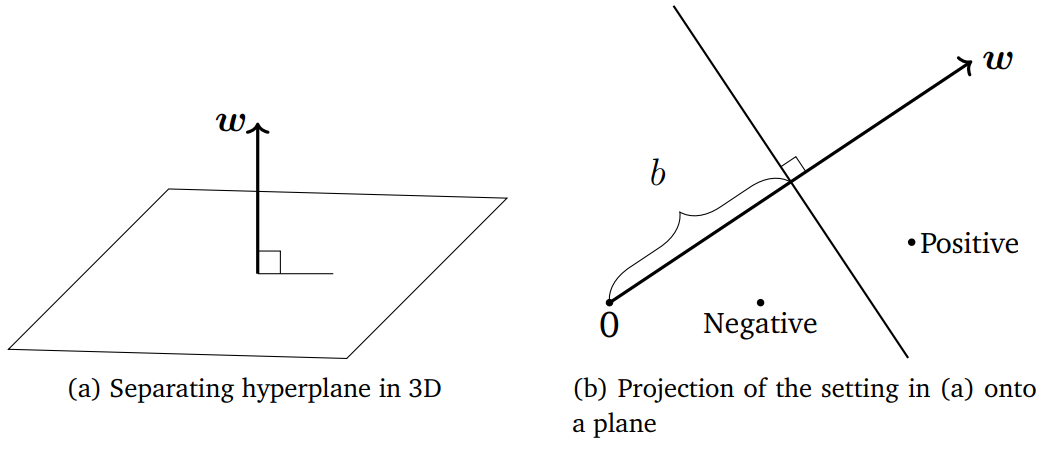
\includegraphics[scale=.3]{figures/hyperplane.png}
           %\caption{caption}
        \end{figure}

    \end{frame}
		}
		
		\begin{frame}{Hyperplane partition: classification}
				Classifying a test example $\mathbf{x}_t$:
				\begin{itemize}
					\item Calculate $f(\mathbf{x}_t):= \mathbf{w}\cdot \mathbf{x}_t + b$ %\pause
					\item Classify $\mathbf{x}_t$ as $+1$ if $f(\mathbf{x}_t)\geq 0$ %\pause
					\item Classify $\mathbf{x}_t$ as $-1$ if $f(\mathbf{x}_t)< 0$ %\pause
				\end{itemize}
				\begin{itemize}
					\item[$\rightarrow$] We must find $\mathbf{w}$ and $b$, such that for all training points holds:
					\begin{itemize}
						\item $f(\mathbf{x}_n)\geq0$ for points having $y_n = +1$
						\item $f(\mathbf{x}_n)<0$ for points having $y_n = -1$
						\item[$\rightarrow$] $y_{n} f(\mathbf{x}_n)\geq0$
					\end{itemize}
				\end{itemize}
			\end{frame}
		
		{ \referencefootnote{Image was taken from \cite{deisenroth_faisal_ong_2020}}
		\begin{frame}{Many candidate hyperplanes}
				Which hypothesis is the best one?
				\begin{figure}
					\center
					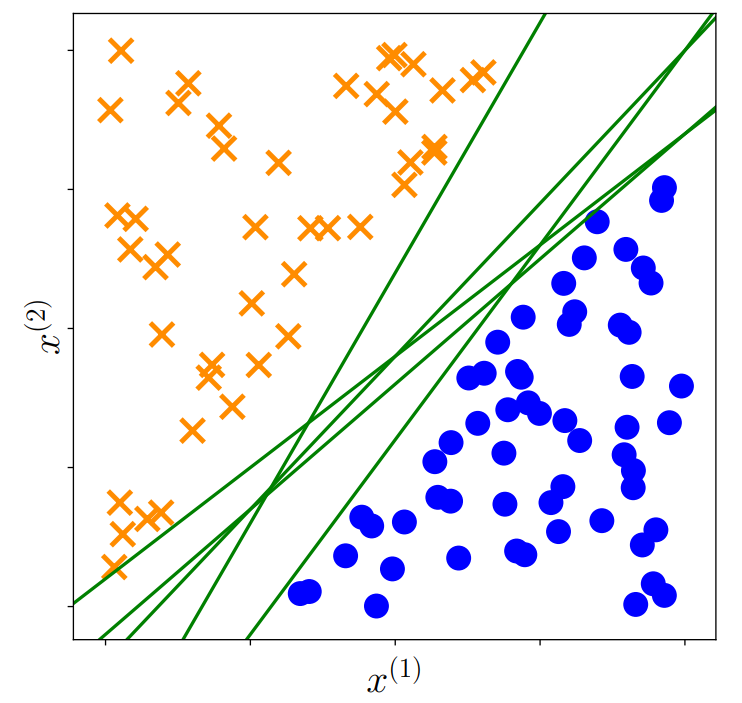
\includegraphics[scale=.2]{figures/binary2.png}
        \end{figure}
				%\pause
				\begin{itemize}
					\item We should try to find the classifier that will give the smallest generalization error!%\pause
					\item Idea: Our classifier should not "favor" any class %\pause
					\item[$\rightarrow$] Choose the hyperplane with equally large (maximum) distance to each class %that maximizes the distance between it and both classes
				\end{itemize}
    \end{frame}
		}

{ \referencefootnote{Image was taken from \cite{deisenroth_faisal_ong_2020}}
    \begin{frame}{The margin}
				What is the distance between a hyperplane and a class?
				
				It is called the \emph{margin} and is defined as the perpendicular distance between the hyperplane and the closest of the data points
				\begin{figure}
					\center
					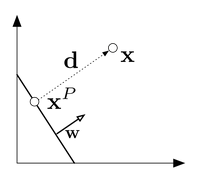
\includegraphics[scale=.6]{figures/margin6.png}
					\caption{If $\mathbf{x}$ is the point closest to the hyperplane, then $\|\mathbf{d}\|_2$ is the margin.}
        \end{figure} %\pause
				It holds:
				\[
				\|\mathbf{d}\|_2 = \frac{|\mathbf{w} \cdot \mathbf{x} + b|}{\|\mathbf{w}\|}
				\]
    \end{frame}
		}
		
		 \begin{frame}{Calculating the margin}
				The margin of $\mathcal{H}$ with respect to the dataset $D$ can be calculated as follows:
				\[
						\gamma(\mathbf{w},b) = \min_{\mathbf{x}\in D}\frac{|\mathbf{w} \cdot \mathbf{x} + b|}{\|\mathbf{w}\|}
				\]
				%\begin{figure}
					%\center
					%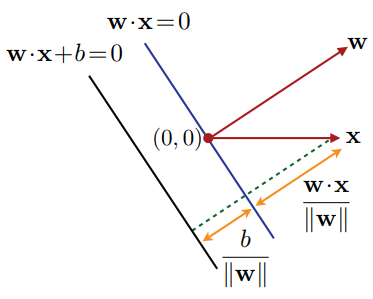
\includegraphics[scale=.4]{figures/margin2.png}
					%\caption{The margin of a point $\mathbf{w}$ in the case $\mathbf{w} \cdot \mathbf{x} > 0$ and $b>0$.}
        %\end{figure}
				\note{Bishop s. 182}
     \end{frame}
		
		
		\begin{frame}{Maximizing the margin}
			%\pause
			We are interested in hyperplanes for which all training points are correctly classified %\pause
			\begin{itemize}
				\item[$\rightarrow$] $y_{n} f(\mathbf{x}_n)\geq 0$ must hold for our margin! %\pause
			\end{itemize}
			Thus, the maximum margin solution is found by solving
			
			 $\underset{\mathbf{w},b}{\argmax}\,\gamma(\mathbf{w},b) $ or %\pause
			
			$\underset{\mathbf{w},b}{\argmax}\, \left\{\frac{1}{\|\mathbf{w}\|}\underset{\mathbf{x}\in D}{\min}\, |\mathbf{w} \cdot \mathbf{x} + b|\right\}$ %\pause
			
			subject to $y_{n}(\mathbf{w} \cdot \mathbf{x} + b)\geq 0$, for all $n = 1, \dots,N$.
			
    \end{frame}
		
    \begin{frame}{Maximizing the margin (2)}
			\begin{itemize}
				\item Observation 1: Above optimizaiton problem is too complex to solve %\pause
				\item Observation 2: Rescaling $\mathbf{w} \rightarrow c\mathbf{w}$ and $b\rightarrow cb$ would not change the distance from the hyperplane to any point %\pause
			\end{itemize}
			$\rightarrow$ We can restrict ourselves to pairs $(\mathbf{w},b)$ scaled such that $\underset{\mathbf{x}\in D}{\min}\, |\mathbf{w} \cdot \mathbf{x} + b| = 1$ %\pause
			
			We can combine this constraint with the previous ones. %\pause
			
			In this case all training points will have to satisfy the constraints: $y_{n}(\mathbf{w} \cdot \mathbf{x}_n + b) \geq 1$:
        %\begin{figure}
					%\center
					%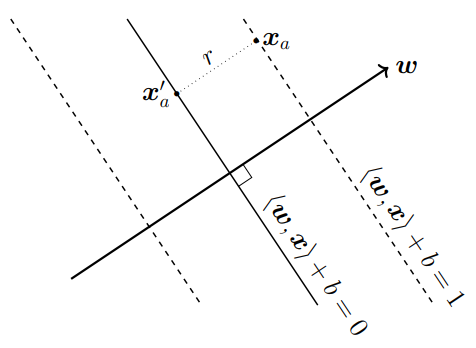
\includegraphics[scale=.3]{figures/margin3.png}
           %%\caption{caption}
        %\end{figure}
    \end{frame}
		
		\begin{frame}{Maximizing the margin (3)}
			Combining the margin maximization with the fact that the examples need to be on the correct side of the hyperplane gives us
			
			$\underset{\mathbf{w},b}{\argmax}\, \frac{1}{\|\mathbf{w}\|}$,
			
			subject to $y_{n}(\mathbf{w} \cdot \mathbf{x} + b)\geq 1$, for all $n = 1, \dots,N$. %\pause
			
			Instead of maximizing the reciprocal of the norm, we often minimize the squared norm:
			
			$\underset{\mathbf{w},b}{\argmin}\,\|\mathbf{w}\|^2$,
			
			subject to $y_{n}(\mathbf{w} \cdot \mathbf{x} + b)\geq 1$, for all $n = 1, \dots,N$. %\pause
			
			$\rightarrow$ This optimization problem is known as the \emph{hard margin SVM}.
    \end{frame}
		
		%\begin{frame}{Solving hard margin SVM}
		%We introduce $N$ Lagrange multipliers $\alpha_n\geq 0$: one for each of the constraints, giving the Lagrangian function
		%\[
			%L(\mathbf{w},b,\boldsymbol{\alpha}) = \frac{1}{2}\|\mathbf{w}\|^2 - \sum_{n=1}^N\alpha_n [y_{n}(\mathbf{w} \cdot \mathbf{x}_n + b)-1]
		%\]
		%where $\boldsymbol{\alpha} = (\alpha_1,\dots,\alpha_N)^{\top}$.
%
			%Note: We are minimizing with respect to $\mathbf{w}$ and $b$ and maximizing with respect to $\boldsymbol{\alpha}$.
    %\end{frame}
		%
		%\begin{frame}{Zero out the derivatives}
			%Partial derivatives of $L(\mathbf{w},b,\boldsymbol{\alpha})$ at a minimum are equal to zero. We get
			%\begin{align*}
				%&\frac{\delta L}{\delta\mathbf{w}} = \mathbf{w} - \sum_{n=1}^N\alpha_n y_{n}\mathbf{x}_n = 0\\
				%&\frac{\delta L}{\delta b} = \sum_{n=1}^N\alpha_n y_{n} = 0
			%\end{align*}
			%
			%Thus we obtain the following conditions:
			%\[
			%\mathbf{w} = \sum_{n=1}^N\alpha_n y_{n}\mathbf{x}_n,\quad 0 = \sum_{n=1}^N\alpha_n y_{n}
			%\]
    %\end{frame}
		%
		%\begin{frame}{Primal vs. dual formulation}
			%The Lagrangian function $L(\mathbf{w},b,\boldsymbol{\alpha})$ is the \emph{primal} form of the optimization problem.
			%
			%We will solve our optimization problem by solving for the \emph{dual} of our original problem.
			%
			%Lagrangian dual problem: Instead of minimizing over $\mathbf{w},b$ subject to constraints involving $\alpha$'s, we can maximize over $\boldsymbol{\alpha}$ (the dual variable) subject to the conditions obtained for $\mathbf{w}$ and $b$:
			%\[
			%\mathbf{w} = \sum_{n=1}^N\alpha_n y_{n}\mathbf{x}_n,\quad 0 = \sum_{n=1}^N\alpha_n y_{n}
			%\]
			%\note{An der Tafel schreiben, wie man mit den conditions primal in dual ueberfuehrt.}
    %\end{frame}
		%
		%\begin{frame}{Dual formulation}
			%Eliminating $\mathbf{w}$ and $b$ from $L(\mathbf{w},b,\boldsymbol{\alpha})$ using our conditions gives us the dual representation od the maximum margin problem, where we maximize
			%\[
			%\widetilde{L}(\boldsymbol{\alpha}) = \sum_{i=1}^N\alpha_i - \frac{1}{2}\sum_{i=1}^N\sum_{j=1}^N\alpha_i\alpha_j y_i y_j (\mathbf{x}_i\cdot \mathbf{x}_j)
			%\]
			%with respect to $\boldsymbol{\alpha}$ subject to the constraints
			%\begin{align*}
				%a_n &\geq 0, \quad n = 1,\dots, N,\\
				%\sum_{n=1}^N\alpha_n y_n &= 0.
			%\end{align*}
    %\end{frame}
		%
		%\begin{frame}{Why the dual formulation?}
        %If the number of features (dimension $m$ of the data points) is greater that the number of the trainig examples, then the dual formulation is advantageous.
				%
				%More important: the dual formulation helps solving linearly non-separable classification problems.
    %\end{frame}
		
		{ \referencefootnote{Image was taken from \cite{LakshmanNaika2019HandwrittenEC}}
		\begin{frame}{Solving hard margin SVM}
			Hard margin SVM is a convex quadratic programming (QP) problem. %\pause
			
			A variety of commercial and open-source solvers are available for solving convex QP problems. %\pause
				\begin{figure}
					\center
					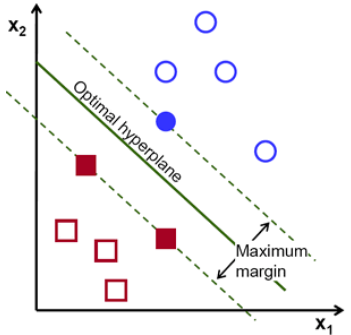
\includegraphics[scale=.32]{figures/margin5.png}
           \caption{Maximum-margin hyperplane solution. Dashed lines are the marginal hyperplanes. The points on them are support vectors.}
        \end{figure}
				
				Support vectors satisfy $y_n(\mathbf{w}\cdot\mathbf{x}_n + b)=1$.
			
			%
			%The solution $\boldsymbol{\alpha}$ the dual problem can be used directly to obtain the $\mathbf{w}$ via
			%\[
				%\mathbf{w} = \sum_{n=1}^N\alpha_n y_{n}\mathbf{x}_n
			%\]
			%In order to classify new data points $\mathbf{x}$ using the trained model, we evaluate the sign of $f(\mathbf{x})$:
			%\[
				%f(\mathbf{x}) = \sum_{n=1}^N\alpha_n y_n (\mathbf{x}\cdot \mathbf{x}_n) + b
			%\]
			%
			%What about $b$?
			%\note{an der tafel die herleitung fuer $f(\mathbf{x})$ zeigen}
    \end{frame}
		}
		
		
				%\begin{frame}{Support vectors}
					%It can be shown that our constraint optimization satisfies the \emph{Karush-Kuhn-Tucker} (KKT) conditions. 
					%
					%$\rightarrow$ The following holds: $\forall n:\alpha_n[y_n(\mathbf{w}\cdot\mathbf{x}_n + b)-1] = 0$
					%
					%$\Rightarrow \alpha_n = 0 \vee y_n(\mathbf{w}\cdot\mathbf{x}_n + b)=1$. 
					%
					%Any data point for which $\alpha_n = 0$ will play no role in the predictions for new data points.
					%The remaining data points are called \emph{support vectors}.
					%
					%Since support vectors satisfy $y_n(\mathbf{w}\cdot\mathbf{x}_n + b)=1$, they correspond to points that lie on the maximum margin hyperplanes in feature space.
					%
    %\end{frame}
		%
						%\begin{frame}{Support vectors (2)}
					%
					%Support vectors lie on the marginal hyperplanes $\mathbf{w}\cdot\mathbf{x}_n + b = \pm 1$.
					%\begin{align*}
						%&\Rightarrow y_n \left( \sum_{i\in \mathcal{S}} \alpha_i y_i (\mathbf{x}_n\cdot \mathbf{x}_i) + b \right)=1\\
						%&\Rightarrow b = \frac{1}{N_{\mathcal{S}}}\sum_{i\in \mathcal{S}} \left(y_i - \sum_{j\in \mathcal{S}} \alpha_j y_j (\mathbf{x}_i\cdot \mathbf{x}_j) \right) 
					%\end{align*}
					%where $\mathcal{S}$ denotes the set of indices and $N_{\mathcal{S}}$ is the total number of support vectors.
        %\begin{figure}
					%\center
					%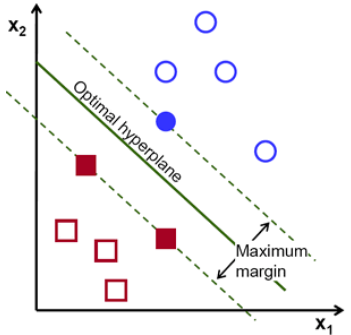
\includegraphics[scale=.35]{figures/margin5.png}
           %\caption{Maximum-margin hyperplane solution. Dashed lines are the marginal hyperplanes. The points on them are support vectors.}
        %\end{figure}
    %\end{frame}
		
		\section{Soft-margin SVM}
			\begin{frame}{What hyperplane best separates this data?}
			  \begin{figure}
					\center
					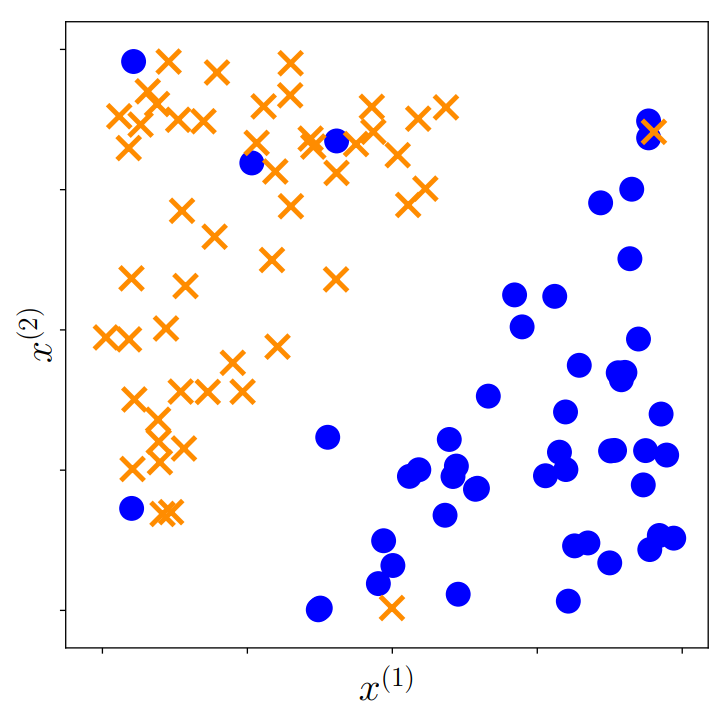
\includegraphics[scale=.25]{figures/binary3.png}
           %\caption{Linear separation is possible, but with some errors.}
        \end{figure} %\pause
				Linear separation is possible, but with some errors.
			\end{frame}

{ \referencefootnote{Image was taken from \cite{deisenroth_faisal_ong_2020}}
			\begin{frame}{Slack variable}
			To be able to deal with noise, we can soften the hard constraints of our optimization and allow for some slack
			  \begin{figure}
					\center
					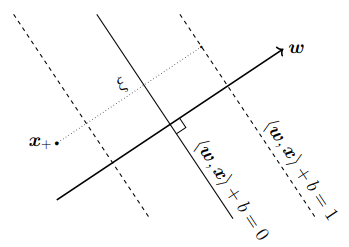
\includegraphics[scale=.45]{figures/slack.png}
           \caption{Slack variable $\xi$ measures the distance of an example $\mathbf{x}_+$ when it is on the wrong side.}
        \end{figure}
			\end{frame}
			}
			
			\begin{frame}{Soft-margin SVM problem}
			$\underset{\mathbf{w},b}{\argmin}\, \|\mathbf{w}\|^2 + C \sum_{n=1}^N \xi_n$,
			
			subject to $y_{n}(\mathbf{w} \cdot \mathbf{x} + b)\geq 1 - \xi_n$, for all $n = 1, \dots,N$.
			
			and $\xi_n \geq 0$, for all $n = 1, \dots,N$. %\pause
			
			The parameter $C$ is a hyperparameter that controls the regularization.
			\end{frame}
		
		\section{Non-Linearly Separable Data}
			{ \referencefootnote{Image was taken from \cite{mohri_fom}}
			\begin{frame}{What hyperplane best separates this data?}
			  \begin{figure}
					\center
					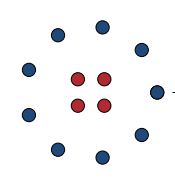
\includegraphics[scale=.6]{figures/nonlinear3.png}
           %\caption{Linear separation is not possible!}
        \end{figure}
				%\pause
				Linear separation is not possible!
			\end{frame}
			}
			%\begin{frame}{Transformation for separation}
				%\begin{figure}
					%\center
					%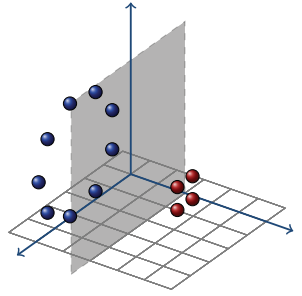
\includegraphics[scale=.5]{figures/nonlinear4.png}
           %\caption{Transforming the points into higher dimensional space makes linear separation possible.}
        %\end{figure}
			%\end{frame}
			{ \referencefootnote{Image was taken from \cite{mohri_fom}}
			\begin{frame}{Transformation for separation}
				While the data may not be linear separable in the input space, it may be in a feature space, after a fancy transormation $\phi$:
				\begin{figure}
					\center
					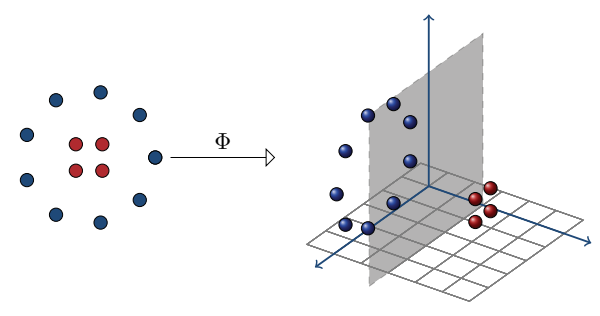
\includegraphics[scale=.5]{figures/nonlinear5.png}
					\caption{Left: the input space. Right: the feature space.}
        \end{figure}
				%\note{figure von transform und transform1 an der tafel malen und erklaeren}
			\end{frame}
			}
				
			\begin{frame}{Non-linear SVM}
				Idea: instead of tweaking the definition of SVM to accomodate non-linear decision boundaries, gain linearly separation by mapping the input data to a higher dimensional feature space, where the classes are linearly separable: %\pause
				\begin{itemize}
					\item Apply transform $\phi:\mathbb{R}^m\rightarrow \mathbb{R}^{D}$ on training data
					\[
					\mathbf{x} = (x_1,\dots,x_m)^{\top} \mapsto \phi(\mathbf{x}) = (\phi_1,\dots,\phi_{D})
					\]
					where $D > m$. %\pause
					\item Train an SVM on the transformed data:
					\[
						\{(\phi(\textbf{x})_1,y_1), \dots, (\phi(\textbf{x})_N,y_N)\}
					\]					
				\end{itemize}
				\note{figure von transform und transform1 an der tafel malen und erklaeren}
			\end{frame}
			
			\begin{frame}{Optimization problem}
        Using the transformations we now need to maximize the following dual Lagrangian:
			\[
			\widetilde{L}(\boldsymbol{\alpha}) = \sum_{i=1}^N\alpha_i - \frac{1}{2}\sum_{i=1}^N\sum_{j=1}^N\alpha_i\alpha_j y_i y_j (\phi(\mathbf{x}_i) \cdot \phi(\mathbf{x}_j))
			\]
			%\pause
			Problem: 
			\begin{itemize}
				\item Dimension $D$ of the feature space can be very large in practice %\pause
				\item Determining the hyperplane solution requires multiple inner product computations in this high dimensional feature space, which can be very costly %\pause
				\item[$\rightarrow$] Use the kernel trick!
			\end{itemize}
			\note{example von FOML s 106 erzaehlen}
			\end{frame}
			
			\section{The Kernel Trick}
			\begin{frame}{Inner products}
        Recall: Training an SVM involves maximizing the following function:
			\[
			\widetilde{L}(\boldsymbol{\alpha}) = \sum_{i=1}^N\alpha_i - \frac{1}{2}\sum_{i=1}^N\sum_{j=1}^N\alpha_i\alpha_j y_i y_j (\phi(\mathbf{x}_i) \cdot \phi(\mathbf{x}_j))
			\]
			%\pause
			We need to compute the inner products $\phi(\mathbf{x}_i) \cdot \phi(\mathbf{x}_j)$ in the feature space. %\pause
			
			We are not really interested in the quantities $\phi(\mathbf{x}_i)$ as such! %\pause
			
			$\rightarrow$ Instead of explicitly defining a non-linear feature map $\phi$ and computing the resulting inner product, we define a similarity function $K(\mathbf{x}_i,\mathbf{x}_j) $ between $\mathbf{x}_i$ and $\mathbf{x}_j$, which implicitly defines $\phi$.
			\end{frame}
			
			\begin{frame}{Kernel function}
        Given a transformation $\phi:\mathbb{R}^m \rightarrow \mathbb{R}^{D}$ from input space $\mathbb{R}^m$ to feature space $\mathbb{R}^D$, the function $K:\mathbb{R}^m \times \mathbb{R}^m \rightarrow \mathbb{R}$ defined by
				\[
				K(\mathbf{x}_i,\mathbf{x}_j) = \phi(\mathbf{x}_i)\cdot \phi(\mathbf{x}_j),\quad \mathbf{x}_i,\mathbf{x}_j \in \mathbb{R}^{m}
				\]
				is called the \emph{kernel function} of $\phi$. %\pause
				
				Generally: kernel function may refer to any function $K:\mathbb{R}^m \times \mathbb{R}^m \rightarrow \mathbb{R}$ that measures the similarity of vectors in $\mathbb{R}^m$ without explicitly defining a transform $\phi$.
				\note{vlt. erklären, wie skalarprodukt als similarity measure genutzt werden kann}
			\end{frame}
			
			\begin{frame}{Kernel function for optimization}
			
			For a choice of kernel $K(\mathbf{x}_i,\mathbf{x}_j) = \phi(\mathbf{x}_i)\cdot \phi(\mathbf{x}_j)$ we train an SVM by maximizing
       			\[
			\widetilde{L}(\boldsymbol{\alpha}) = \sum_{i=1}^N\alpha_i - \frac{1}{2}\sum_{i=1}^N\sum_{j=1}^N\alpha_i\alpha_j y_i y_j K(\mathbf{x}_i,\mathbf{x}_j)
			\]
			
			Computing $K(\mathbf{x}_i,\mathbf{x}_j)$ can be done without computing the mappings $\phi(\mathbf{x}_i)$ and $\phi(\mathbf{x}_j)$.
			
			This way of training a SVM in feature space without explicitly computing the mappings $\phi$ is called the \emph{kernel trick}. 
			\end{frame}
			
			\begin{frame}{Example}
        Define $\phi:\mathbb{R}^2 \rightarrow \mathbb{R}^6$ by
				\[
				\phi((x_1,x_2)^{\top}) = (x_1^2,x_2^2,\sqrt{2}x_1^2 x_2^2, \sqrt{2}x_1^2,\sqrt{2}x_2^2, 1)^{\top}
				\]
				The inner product in the feature space is
				\[
				\phi((x_1,x_2)^{\top})\cdot \phi((x^{'}_1,x^{'}_2)^{\top}) = (x_1 x_1^{'} + x_2 x_2^{'}+ 1)^2
				\]
				Thus, we can directly define a kernel function $K:\mathbb{R}^2 \times \mathbb{R}^2 \rightarrow \mathbb{R}$ by
				\[
				K(\mathbf{x}_1,\mathbf{x}_2) = (x_1 x_1^{'} + x_2 x_2^{'}+ 1)^2
				\]
			\end{frame}
			
			{ \referencefootnote{Image was taken from \cite{mohri_fom}}
			\begin{frame}{Example: XOR function}
        \begin{figure}
					\center
					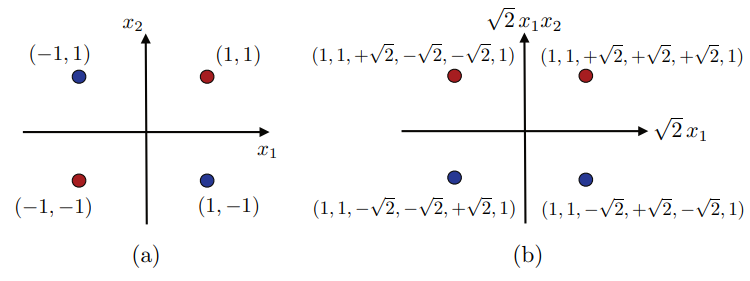
\includegraphics[scale=.5]{figures/xor.png}
           \caption{(a) XOR Problem linearly non-separable in the input space. (b) Points are mapped to the six-dimensional space defined by second degree polynomial (here projection of these points on the two-dimensional space defined by their third and fourth coordinates). The problem becomes separable by the hyperplane $x_1x_2 = 0$.}
        \end{figure}
			\end{frame}
			}
			
			\begin{frame}{Useful kernel functions}
				\begin{itemize}
					\item Polynomial kernel: 
					\[
					K(\mathbf{x}_1,\mathbf{x}_2) = (\mathbf{x}_1 \cdot \mathbf{x}_2 + 1)^d
					\]
					where $d$ denotes the degree of the polynomial and is a hyperparameter.
					\item Gaussian kernel:
					\[
					K(\mathbf{x}_1,\mathbf{x}_2) = exp\left(-\frac{\|\mathbf{x}_1 - \mathbf{x}_2 \|^2}{2\sigma^2} \right)
					\]
					where $\sigma$ is a hyperparameter.
					\item Sigmoid kernels:
					\[
					K(\mathbf{x}_1,\mathbf{x}_2) = tanh(a(\mathbf{x}_1 \cdot\mathbf{x}_2)+b)
					\]
					where $a$ and $b$ are hyperparameters.
					\end{itemize}
			\end{frame}
			
			{ \referencefootnote{Image was taken from \cite{deisenroth_faisal_ong_2020}}
			\begin{frame}{Example: SVM with Gaussian kernel}
        \begin{figure}
					\center
					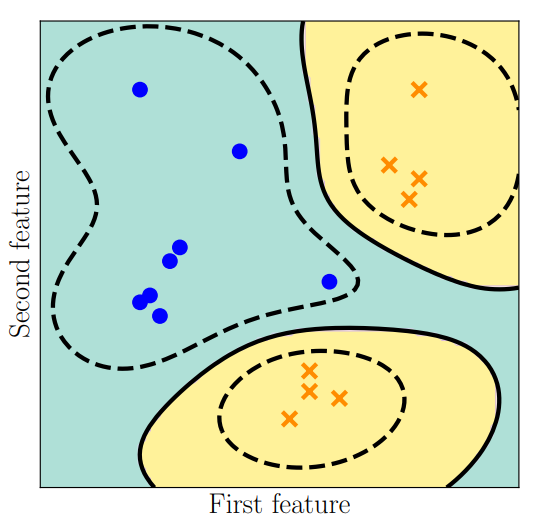
\includegraphics[scale=.5]{figures/kernel1.png}
        \end{figure}
			\end{frame}
			}
			
			{ \referencefootnote{Image was taken from \cite{deisenroth_faisal_ong_2020}}
			\begin{frame}{Example: SVM with polynomial (degree 2) kernel}
        \begin{figure}
					\center
					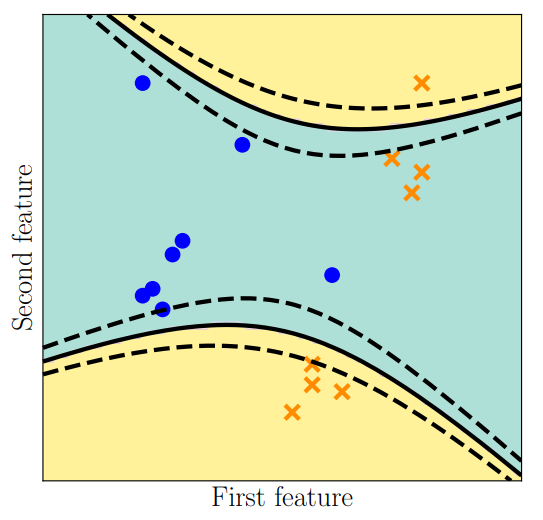
\includegraphics[scale=.5]{figures/kernel2.png}
        \end{figure}
			\end{frame}
			}
			
			{ \referencefootnote{Image was taken from \cite{deisenroth_faisal_ong_2020}}
			\begin{frame}{Example: SVM with polynomial (degree 3) kernel}
        \begin{figure}
					\center
					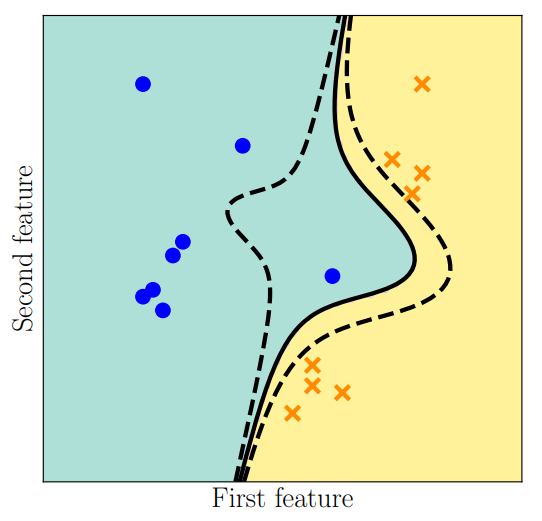
\includegraphics[scale=.5]{figures/kernel3.png}
        \end{figure}
			\end{frame}
			}
			
			\begin{frame}{Choosing suitable kernel functions}
				Kernel function is a hyperparameter. %\pause
				
				The choice depends on a problem at hand. %\pause
				
				Try several common ones and choose the one with the best results on the validation set. %\pause
				
				If in doubt - use a Gaussian!
			\end{frame}
			
			 \begin{frame}{Literature}
    \printbibliography
  \end{frame}
			
\end{document}
